%&program=xelatex
%&encoding=UTF-8 Unicode
% SVN keywords
% $Author: bernardo $
% $Date: 2014-09-19 20:37:55 +0100 (Fri, 19 Sep 2014) $
% $Revision: 6678 $
% $URL: http://metis.ipfn.ist.utl.pt:8888/svn/cdaq/Users/Bernardo/Aulas/LFEB/teXfiles/Pendulo/pendulo_gravitico.tex $
\documentclass[a4paper,twoside,12pt]{article}      % Comments after  % are ignored
%\usepackage{hyperref}                 % For creating hyperlinks in cross references
%\documentclass[a4paper,12pt]{article} 
%

\usepackage{ifxetex}% for XELATEX, or PDFlatex
\usepackage{ifplatform} 
%
\ifxetex
\usepackage{polyglossia} \setmainlanguage{portuges}
\usepackage{fontspec}
\ifwindows
\setmainfont[Ligatures=TeX]{Garamond}
\setsansfont[Ligatures=TeX]{Gill Sans MT}
	\setmonofont[Scale=0.95]{Courier}
	%\setmonofont[Scale=MatchLowercase]{Courier}	
\fi
\iflinux
\setmainfont[Ligatures=TeX]{Linux Libertine O}
\setsansfont[Ligatures=TeX,Scale=MatchLowercase]{Linux Biolinum}
\setmonofont[Scale=MatchLowercase]{Courier}
\fi
\ifmacosx
% add settings
\fi
%
\usepackage{xcolor,graphicx} 
\else
%PdfLaTEX
\usepackage[portuguese]{babel}
\usepackage[utf8]{inputenc}
\usepackage[T1]{fontenc}
\usepackage{graphics}                 % Packages to allow inclusion of graphics
\usepackage{color}                    % For creating coloured text and background
\fi

\usepackage{amsmath,amssymb,amsfonts} % Typical maths resource packages

\oddsidemargin 0cm
\evensidemargin 0cm

\pagestyle{myheadings}         % Option to put page headers
                               % Needed \documentclass[a4paper,twoside]{article}
\markboth{{MEFT}}
{{\small\it \protect\input{../../LIFE.txt}}}

\textwidth 15.5cm
\topmargin -1cm
\parindent 0cm
\textheight 24cm
\parskip 1mm


%\setmainfont[Ligatures=TeX]{Hoefler Text} 
%\setmainfont[Ligatures=TeX]{Times}
%\setsansfont[Ligatures=TeX,Scale=MatchLowercase]{Gill Sans} \setmonofont[Scale=MatchLowercase]{Courier}
%\setromanfont[Numbers=Uppercase]{Hoefler Text}
%\usepackage{xcolor,graphicx} 

%[pdftex]
%\usepackage{amsmath,amssymb} 
%\usepackage{amsmath} 
%\usepackage{textcomp}
%\usepackage{float}

% Math macros
\newcommand{\ud}{\,\mathrm{d}} 
\newcommand{\HRule}{\rule{\linewidth}{0.5mm}}

%\title{ e Difracção de Ondas Electromagnéticas num meio dieléctrico, homogéneo e isotrópico } 
%\subtitle{ aplicação à luz visível} 

\author{Prof. Bernardo B. Carvalho} 

%, Bernardo Brotas Carvalho\\bernardo@ipfn.ist.utl.pt} 
\date{ Setembro 2014} 

\begin{document} 

%	\begin{center}
%	\textsc{\large Laboratório de Física Experimental Básica - MEFT - 2012/2013 }\\%[0.5cm]
%	\end{center}

\includegraphics[width=0.2\textwidth]{../../logo-ist}%\\[1cm]  %%  Logo_IST_color
	
	\HRule \\[0.5cm]
	{ \huge   \bfseries \textsc{ Pêndulo gravítico } }\\[0.4cm]
	{ \large \bfseries Determinação do período do pêndulo simples e aferição do valor da aceleração da gravidade local $g$  }\\
%	{ \large \begin{flushleft}
%	 $\bullet$ Deflexão magnética \\
%	 $\bullet$ Deflexão magnética em equilíbrio com deflexão eléctrica
%	\end{flushleft} }
	\HRule \\%[0.5cm]
%	\textsc{\Large Laboratório de Física Experimental Básica}\\[0.5cm]
	
%	\input{./title_exa.tex} 

%\maketitle
%\section{\sf  Conceitos necessários:} 
%\begin{enumerate}
%	\item Força eléctrica. Campo eléctrico (Electrostático)
%	\item Potencial eléctrico. Equipotencial. Energia potencial eléctrica 
%	\item Condutores e dieléctricos. Condensador plano
%	\item Efeitos da corrente eléctrica estacionária criada por uma espira 	
%	\item Força de Laplace
%\end{enumerate}

\section{\sf Objectivo}

Pretende-se com este trabalho determinar o período de oscilação de um pêndulo simples, constituído por um fio e uma massa, para diferentes comprimentos do fio. A partir destes valores é possível determinar o valor da aceleração da gravidade local $g$.

Este tipo de pêndulos foi estudado extensivamente por Galileu Galilei (1564-1642), no início do séc. XVIII. Galileu foi o primeiro a constatar a propriedade de isocronismo do pêndulo: para pequenas amplitudes de oscilação, o período é independente da amplitude do movimento. Também descobriu que o período não depende do valor da massa, e é proporcional à raiz quadrada do comprimento do fio. Estas propriedades vieram a permitir a utilização do pêndulo como instrumentos para medição de intervalos de tempo: os relógios de pêndulo.


\section{\sf Movimento Harmónico Simples}

O pêndulo gravítico é um exemplo simples de um importante modelo matemático, o ``Oscilador Harmónico'' (OH), de vastíssima utilização em quase todos o ramos da Física,
 bem como muitas áreas de Engenharia. 
 Neste modelo, um sistema físico arbitrário encontra-se na vizinhança de uma posição de equilíbrio, onde há um mínimo (local ou absoluto) da sua energia potencial  ($E_P$), de origem gravítica, elástica, eletrostática ou outra. Este sistema apresenta as seguintes características (ver Figura 1):

\begin{figure}
	[b] \centering 
	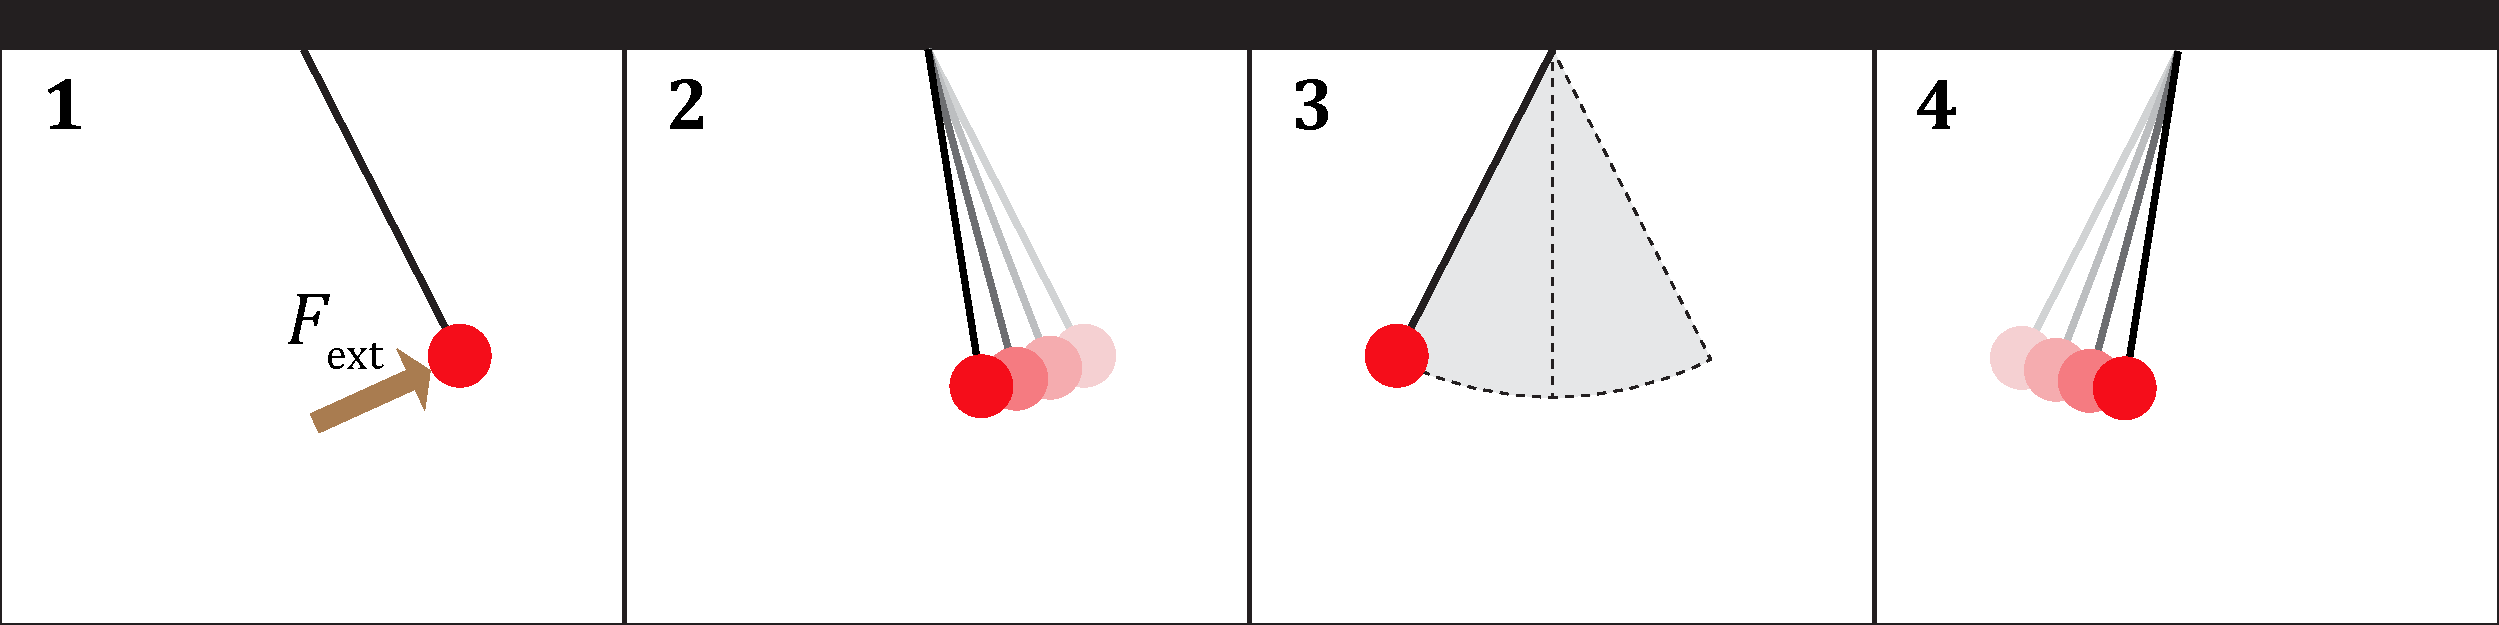
\includegraphics[width=0.9	\textwidth]{Fig-1} 
	\caption{Movimento de um pêndulo gravítico.  \label{fig:1}} 
\end{figure}
 
\begin{enumerate}
\item  Ao distanciar-se deste mínimo, por uma perturbação ou outra qualquer força externa inicial, 
surge uma força de índole conservativa, sempre direcionada de forma a repor o equilíbrio.
\item Quando as forças exteriores deixam de actuar, o sistema adquire movimento, 
transferindo-se a energia potencial para energia cinética ($E_C$).
\item Ao retomar a posição de equilíbrio, o movimento prossegue por inércia até se alcançar um 
novo máximo, normalmente simétrico ao ponto inicial.
\item Na ausência de atrito, o sistema regressa  ao ponto de partida e o ciclo repete-se infinitamente, com período $T_0$ constante (``Oscilador Livre''). Contudo, na presença de forças dissipativas a energia total deixa de ser constante e irá dissipar-se, diminuindo a amplitude do movimento, até desaparecer (``Oscilador Amortecido'').
\end{enumerate}


\subsection{\sf Sistema massa-mola}
Antes de analisarmos o pêndulo gravítico, vamos considerar o modelo de OH mecânico mais simples, que consiste num sistema de uma massa $m$ que se 
move na horizontal e sem atrito,  presa a uma mola de constante elástica $k_{mola}$ que é fixada na sua outra extremidade a um ponto fixo (Figura \ref{fig:2}). 

Pretendemos determinar a função $x(t)$ que descreve o movimento da massa nestas condições. Caso a massa se desloque da posição de equilíbrio ($x =x_0$), a energia potencial elástica aumenta e mola irá exercer uma força de sentido contrário ao do deslocamento $\Delta x \equiv x - x_0$. Por simplicidade faz-se $x_0=0$, e portanto $x=\Delta x$.
 No modelo ideal da mola \emph{linear}  a força é sempre proporcional ao deslocamento $x$:

\begin{figure}
	[b] \centering 
	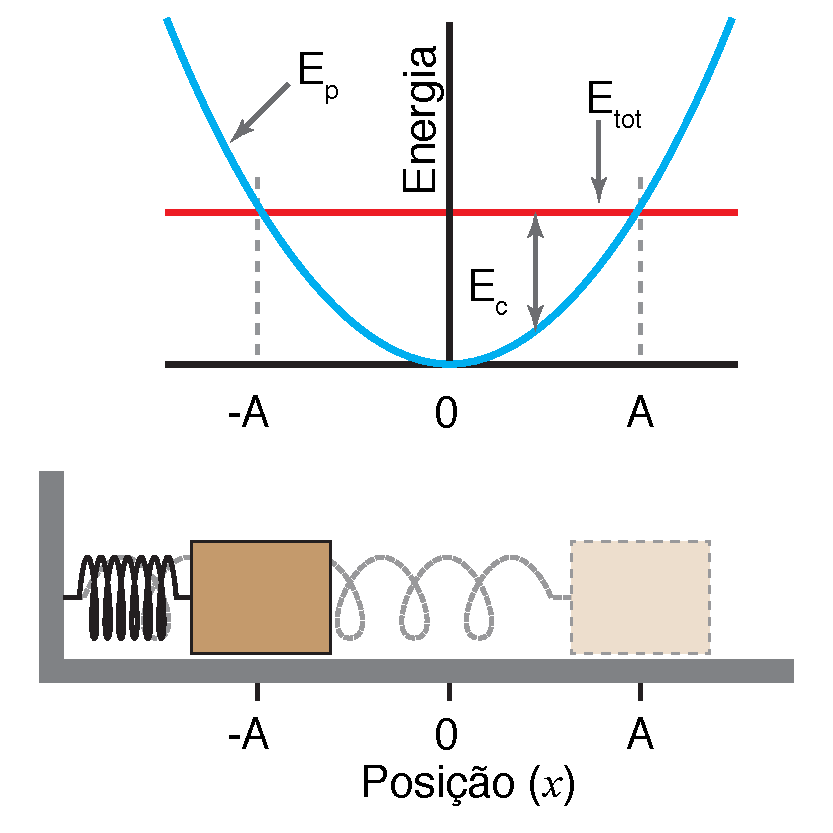
\includegraphics[width=0.4	\textwidth]{harmonic_oscillator} 
	\caption{Oscilador Harmónico Simples \emph{massa-mola}.  \label{fig:2}} 
\end{figure}

\begin{equation}
F_{mola} = - k_{mola} \, x \qquad 
\end{equation}

A partir da segunda equação de Newton, $F=m a$, e sabendo que $ a = \ddot{x}= \frac{d^2 x}{dt^2}$, é possível chegar facilmente  à equação de movimento do sistema massa-mola (equação diferencial de 2.º grau),

\begin{equation}
	\label{eq:1} 
 m a = - k_{mola} x \Leftrightarrow \frac{d^2 x}{dt^2}  + \frac{k_{mola}}{m} x = 0
\end{equation}

%\Rightarrow
Pode-se verificar após alguma álgebra\footnote{Consultar \emph{Notas de apoio às aulas teóricas}} que a seguinte função temporal periódica é solução da equação (\ref{eq:1}):

\begin{equation}
	\label{eq:solu_mola}
x(t) = c_1 \cos(\omega_0 \, t) + c_2 \sin(\omega_0 \, t) = A_0 \sin(\omega_0 \, t + \phi_0) \text{, com } \omega_0 = \sqrt{\frac{k_{mola}}{m}}
\end{equation}

em que $ A_0 $ é a amplitude e $\phi_0$ é a fase, ambas constantes e dependentes da condições (a posição e a velocidade) iniciais. Finalmente $\omega_0$ é a frequência angular de ressonância, inversamente proporcional ao período, o qual depende apenas da massa $m$ e de $k_{mola}$:
%, $\frac{2 \pi}{T}$,

\begin{equation}
	\label{eq:period_mola}
T_0 = \frac{2 \pi}{\omega_0} = 2\pi\; \sqrt{\frac{m}{k_{mola}}}
\end{equation}

Assim, a solução para a posição $x(t)$ é uma função sinusoidal (harmónica). Uma vez que a velocidade $v(t)$ é a derivada temporal da posição, também será uma função sinusoidal, com um desfasamento de $\pi/2$ em relação a $x(t)$.



\subsection{\sf Pêndulo gravítico}
O pêndulo gravítico consiste na sua forma idealizada numa massa pontual suspensa\footnote{No Latim \emph{pendulus}} a partir de um fio inextensível, de comprimento $l$ fixo e de massa desprezável, que pode rodar de um ângulo $\theta$ em torno de um ponto (o eixo, ou pivô). Quando a massa se desvia da posição central $\theta=0$, a força gravítica aplicada (o seu peso $F_g = m \, g $) adquire uma componente $F_{\theta}$ na direcção de movimento (tangente à trajectória circular) e que tende a restabelecer o equilíbrio (Figura \ref{fig:3}).

\begin{figure}
	[!htbp] \centering 
	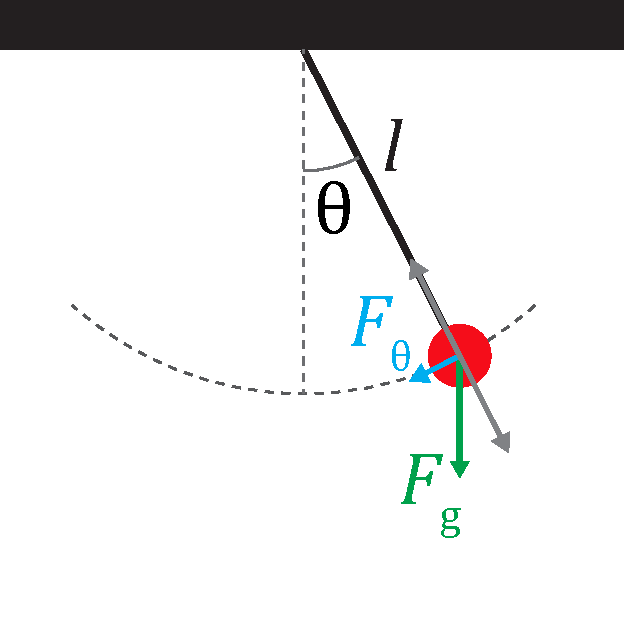
\includegraphics[width=0.4	\textwidth]{Fig-2}
	\caption{Força de gravidade $F_g$ no pêndulo gravítico e a sua projecção $F_{\theta}$ na direcção de movimento. \label{fig:3} } 
\end{figure}

Se a posição do pêndulo for descrita pela coordenada $s= l\cdot \theta$ ao longo da sua trajectória, 
então a força restauradora é 
\begin{equation}
	\label{eq:4} 
F_{\theta} = - F_{g} \sin(\theta) = - mg \sin(\theta)
\end{equation}

e a equação diferencial de movimento para a posição $s$ resulta em
\begin{align}
	\label{eq:5} 
	a &= \frac{d^2 s}{dt^2} =  l\;  \frac{d^2 \theta}{dt^2} \nonumber \\
	ma &= F_{\theta}\Leftrightarrow m \, l \, \frac{d^2 \theta}{dt^2} = - m \,  g \, \sin(\theta) \nonumber \\
	 & \Rightarrow \frac{d^2 \theta}{dt^2} + \frac{g}{l} \sin(\theta) = 0
%l \,\frac{d^2 x}{dt^2} = \frac{k_{mola}}{m} x
\end{align}

Esta equação não tem uma resolução analítica simples, mas através do método  da \emph{linearização} (o ``canivete suíço'' dos físicos),  utiliza-se a aproximação $ \sin(\theta) \simeq \theta$ , válida para  $\theta_0 \le 0.08\,\mathrm{rad}$ (aqui  os ângulos têm de ser medido em radianos!\footnote{ Por exemplo: $\sin(5 ^{\circ}) = \sin(0.08726... \, \mathrm{rad}) = 0.08715... $}).
Com esta aproximação ficamos com 

\begin{equation}
	\label{eq:6} 
	 \frac{d^2 \theta}{dt^2} + \frac{g}{l} \theta =0
\end{equation}

cuja solução matemática é exacta e semelhante à expressão (\ref{eq:solu_mola}),

\begin{equation}
	\label{eq:solu_pend}
\theta (t) = \theta_0 \sin(\omega_0 \, t + \phi_0) \text{, com } \omega_0 = \sqrt{\frac{g}{l}}.
\end{equation}

O que é interessante neste modelo é que o efeito da \emph{massa gravítica } anula o da \emph{massa inercial } e o período do pêndulo $T_0$ fica a  depender apenas do comprimento $l$  e do valor da aceleração da gravidade $g$  local:\footnote{À superfície da Terra e à latitude de Lisboa: $g\approx 9.800\,\mathrm{m s^{-2}}$. Consultar também o Projecto ``Pêndulo Mundial'', baseado no e-lab do IST: http://www.elab.ist.utl.pt/}
%à superfície da Terra $g\approx 9.81\,m s^{-2}$ e $g/\pi^2 \approx 0.994 \,m s^{-2}$}

\begin{equation}
	\label{eq:period_pend}
T_0 = \frac{2 \pi}{\omega_0} = 2\pi\; \sqrt{\frac{l}{g}} \quad  \text{, para }	\theta_0 \ll 1.
\end{equation}
%\simeq

A equação (\ref{eq:period_pend}) representa precisamente a dependência entre o período e o comprimento do pêndulo deduzida por Galileu.
A partir dessa época, estes dispositivos foram sistematicamente utilizados para medir o tempo (e consequentemente a latitude), sendo a base 
de quase todos os relógios de precisão até meados do século passado, com maior ou menor complexidade.
Actualmente apenas os relógios decorativos ou de luxo usam variações do pêndulo\footnote{Mas ainda são úteis para se fazer ciência: Ver por exemplo a revista \emph{Nature} de Julho de 2015, http://www.nature.com/articles/srep11548}.

\subsubsection{A influência do atrito}
Até aqui, desprezámos o atrito do ar no movimento do pêndulo. Ao introduzir esta contribuição, na aproximação de atrito cinético 
proporcional à velocidade, a  equação (\ref{eq:6}) muda para

\begin{equation}
%	\label{eq:6} 
	 \frac{d^2 \theta}{dt^2} + \lambda \, \frac{1}{m}  \frac{d \theta}{dt} + \frac{g}{l} \theta =0 \quad (\lambda \text{ = Coeficiente de atrito viscoso})
\end{equation}

O primeiro efeito, que se pode verificar no laboratório, é na amplitude do movimento $\theta_0$: já não será uma constante, mas irá diminuir inexoravelmente com o tempo. 

O segundo efeito, muito mais difícil de observar, é que existe uma muito pequena alteração no período, que tem agora o valor
\begin{equation}
T_1= T_0 / \sqrt{1 - \zeta^2}, \quad \text{onde }  \zeta = \frac{\lambda}{2\, m} \sqrt{\frac{l}{g}} .
\end{equation}



O factor  $ \zeta $ também se pode relacionar com o factor de amortecimento\footnote{Em engenharia é designado por Factor de Qualidade} $Q$:
\begin{equation}
Q = 2 \pi \times \frac{\text{Energia do Pêndulo}}{\text{Energia perdida num ciclo}}
\end{equation}

Nota final: 
A resolução analítica (infelizmente bastante complexa) da Equação 	(\ref{eq:5})  tem como solução para o período uma série  infinita de potências de $\theta_0$:

\begin{equation}
	\label{eq:period_pend_exa}
T_0 =  2\pi\, \sqrt{\frac{l}{g}} \left(1 + \frac{1}{16} \theta_0^{2} + \frac{11}{3072} \theta_0^{4} +
 \frac{737280}{3072} \theta_0^{6} + \frac{22931}{1321205760} \theta_0^{8} + \cdots \right)
\end{equation}

Naturalmente, verifica-se imediatamente que na aproximação $\theta_0 \ll 1$ a Equação \ref{eq:period_pend} continua válida.




\newpage
\section{\sf Procedimento Experimental}
{ \large Material }
 \begin{flushleft}
	 $\bullet$ Suporte do pêndulo \\
	 $\bullet$ Massas esféricas de chumbo, linha (quase) inextensível de nylon e com massa desprezável \\
	 $\bullet$ Régua graduada, cronómetro, fita métrica, transferidor, balança
\end{flushleft} 

\begin{enumerate}
\item Comece a sessão de laboratório estimando a precisão que obtém na medição do tempo com o cronómetro, tendo em conta 
o tempo de reacção do corpo humano. 
Com a ajuda de um colega e de uma régua graduada, obtenha 15 medidas da distância de queda da régua. 
\item A partir da média das distâncias $\overline{D}$ e do respectivo desvio padrão obtenha\footnote{Considere $\,\overline{t}=\sqrt{\frac{2 \overline{D}}{g}}$ e   
$e_{\overline{t}}=\sqrt{\frac{2 }{g}} \cdot \frac{1}{2\sqrt{\overline{D}}} \cdot e_{\overline{D}}= \overline{t} \cdot \frac{1}{2\overline{D}} \cdot e_{\overline{D}} $ } o seu tempo de reacção $\overline{t}$ e a respectiva incerteza $e_{\overline{t}}$. 
\item Repita para cada um dos demais elementos do grupo e preencha uma tabela semelhante à ilustrada.
\begin{center}
\begin{tabular}{|r|c|c|c|}
\hline
Ensaio  & $D_A$ - Distância & $D_B$ - Distância & $D_C$ - Distância  \\
\# & de queda (cm) & de queda (cm) & de queda (cm)\\
\hline \hline
1 & & & \\
\hline
2 & &  &\\
\hline ... & & & \\
%\hline 4 & & & \\
\hline 15 & & & \\
\hline \hline
Média $\overline{D}$ (m) & &  & \\
Desvio padrão (m) & & & \\
Erro da média  $e_{\overline{D}}$ (m) & & & \\ 
Tempo de reacção $\overline{t} \pm e_{\overline{t}}$ (s) & $\qquad \pm$  & $\qquad \pm$  & $\qquad \pm$  \\
\hline
\end{tabular}
\end{center}

\item Monte o sistema de pêndulo gravítico e obtenha o período para diversos comprimentos do fio. 
\item Obtenha o valor de $g_{exp}$ para estes ensaios, usando a expressão (9), bem como a respectiva incerteza experimental. 
\item Compare o valor final de $g_{exp}$ obtido com o valor tabelado $g_{tab}$ e estime o desvio à exactidão que obteve. 
\end{enumerate}

\smallskip

\subsection{\sf Aspectos a ter em conta:}

 \begin{flushleft}
	 $\bullet$ Uma massa pendurada num fio tem mais que o grau de liberdade em $\theta$. Tente assegurar-se de que o pêndulo oscila apenas ao longo de um plano. \\
	 $\bullet$ Tente minimizar o efeitos de paralaxe na determinação dos ângulos.\\
	 $\bullet$ Naturalmente, a massa utilizada não é pontual. Quais os erros sistemático e aleatório na medida do comprimento $l$? \\	
	 $\bullet$ Como pode minimizar a incerteza da medição do período? Medindo o tempo num ou em vários ciclos? \\
\end{flushleft} 

\subsection{\sf Actividades adicionais (se houver tempo):}

 \begin{flushleft}
	 $\bullet$ Verifique experimentalmente que o período do pêndulo não depende do valor da massa.\\
	 $\bullet$ Verifique experimentalmente que para grandes ângulos iniciais, o período do pêndulo varia. Aumenta ou diminui?\\
%	 Para que valores de $\theta_0$ o valor calculado de $g_{exp}$ se afasta de $\overline{g_{exp}}$ com desvio de $0.05$ ?\\
	 $\bullet$ Tente estimar a energia que se perde em cada ciclo (em percentagem) devido ao atrito.\\
	 $\bullet$ Qual o comprimento do fio para construir um relógio pendular com período de $1$ s? 
	 E se fosse na superfície da Lua? ($M_{Lua}=0,0123 M_{Terra}, R_{Lua}=0,273 R_{Terra}$)\\
	 $\bullet$ Utilize o equipamento digital de detecção da passagem da massa para medir o período do pêndulo (para um comprimento apenas), e compare com os valores obtidos manualmente.
\end{flushleft} 

%\textbf{Ver descrição no guia de laboratório pgs.77-81}

\end{document} 	

